\documentclass[aspectratio=169]{beamer}

% ---------- ENCODING & FONTS ----------
\usepackage[utf8]{inputenc}
\usepackage[T1]{fontenc}

% ---------- THEME & LOOK ----------
\usetheme{Madrid}
\usecolortheme{seahorse}
\usefonttheme{professionalfonts}
\setbeamertemplate{navigation symbols}{}
\setbeamercovered{transparent}
\setbeamertemplate{itemize items}[circle]
\setbeamertemplate{enumerate items}[default]
\setlength{\parskip}{0.25em}

% ---------- COLORS ----------
% Beamer already loads xcolor, so we just define our colors
\definecolor{accent}{RGB}{0,92,184}
\definecolor{soft}{RGB}{233,244,255}
\definecolor{lightred}{RGB}{245,210,210}
\setbeamercolor{structure}{fg=accent}
\setbeamercolor{title}{fg=white,bg=accent}
\setbeamercolor{frametitle}{fg=accent}
\setbeamercolor{block title}{bg=accent!12,fg=accent}
\setbeamercolor{block body}{bg=soft}

% ---------- PACKAGES ----------
\usepackage{booktabs}
\usepackage{amsmath, amssymb}
\usepackage{array}
\usepackage{multirow}
\usepackage{hyperref}
\hypersetup{colorlinks=true,linkcolor=accent,urlcolor=accent}

% ---------- SAFE TRANSITION FALLBACK ----------
\makeatletter
\@ifundefined{transfade}{\newcommand{\transfade}[1][]{}}{}
\makeatother

% ---------- PLACEHOLDER BOX FOR FIGURES ----------
\newcommand{\placeholderbox}[2][0.82\linewidth]{%
  \begin{center}
    \fbox{\begin{minipage}[c][0.46\textheight][c]{#1}
      \centering \vspace{0.3em}
      \textbf{#2}\\[0.6em]
      \emph{Insert figure/diagram here later.}
    \end{minipage}}
  \end{center}
}

% ---------- TITLE ----------
\title{\textbf{Where Prices Come From: The Interaction of Supply and Demand \vspace{.5cm}\\  }}
\subtitle{ {\large ECON 101 - Macroeconomics}}
%\institute{UNBC}
\author{Muhebullah Karimzada}
\date{Winter 2026}



\begin{document}

% ============================================================
% TITLE
% ============================================================
\begin{frame}[plain]
  \titlepage
\end{frame}

% ============================================================
\begin{frame}{Chapter Outline}
\transfade
\begin{itemize}
  \item \textbf{3.1} The Demand Side of the Market
  \item \textbf{3.2} The Supply Side of the Market
  \item \textbf{3.3} Market Equilibrium: Putting Buyers and Sellers Together
  \item \textbf{3.4} The Effect of Demand and Supply Shifts on Equilibrium
\end{itemize}
\end{frame}

% ============================================================
\section{The Demand Side of the Market (3.1)}
% ============================================================

\begin{frame}{3.1 Learning Objective}
\transfade
\begin{block}{Goal}
Discuss the variables that influence demand.
\end{block}
\begin{itemize}
  \item We begin by investigating how \textbf{buyers} behave.
  \item \textbf{Market demand:} the demand by all the consumers of a given good or service.
  \item Key tools:
  \begin{itemize}
    \item Demand schedule
    \item Demand curve
  \end{itemize}
\end{itemize}
\end{frame}

\begin{frame}{Figure 3.1 -- A Demand Schedule and Demand Curve (1 of 3)}
\transfade
\begin{itemize}
  \item \textbf{Demand schedule:} a table that shows the relationship between the \textbf{price} of a product and the \textbf{quantity of the product demanded}.
  \item \textbf{Demand curve:} a curve that shows the relationship between the price of a product and the quantity of the product demanded.
\end{itemize}
\end{frame}

\begin{frame}{Figure 3.1 -- A Demand Schedule and Demand Curve }
\centering
\vspace{2em}

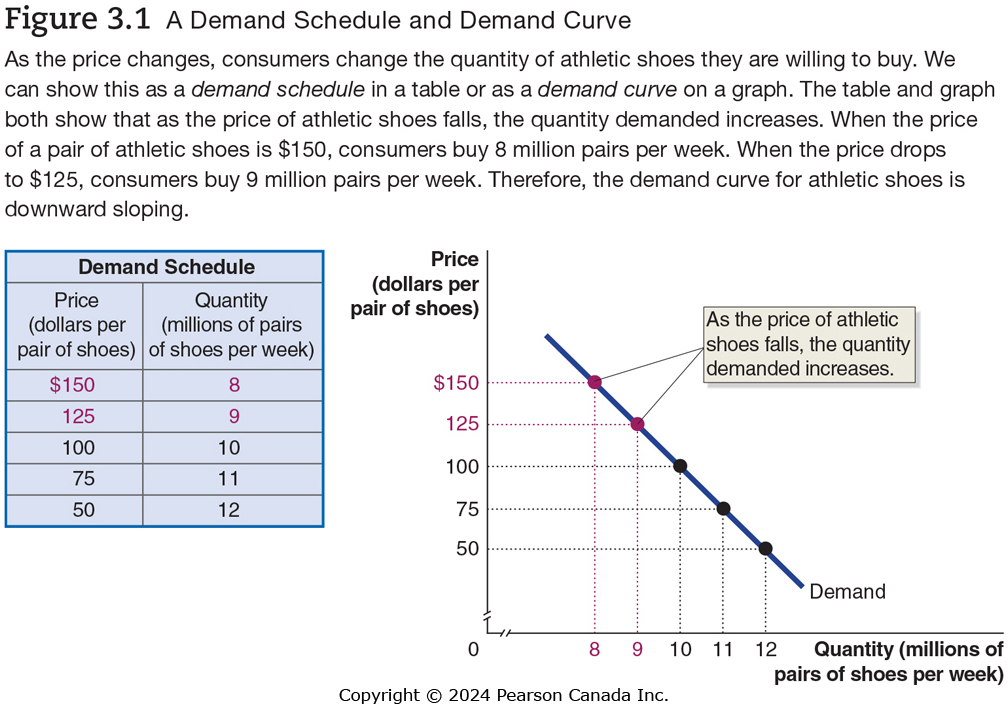
\includegraphics[width=0.63\linewidth]{Fig03-001}.
\end{frame}

\begin{frame}{Figure 3.1 -- Demand Curve and Ceteris Paribus (2 of 3)}
\transfade
\begin{itemize}
  \item When drawing the demand curve, we assume \textbf{ceteris paribus}.
  \item \textbf{Ceteris paribus} (``all else equal'') condition:
  \begin{itemize}
    \item When analyzing the relationship between two variables (such as price and quantity demanded), \textbf{other variables must be held constant}.
  \end{itemize}
\end{itemize}
\end{frame}

\begin{frame}{Figure 3.1 -- Quantity Demanded and the Law of Demand (3 of 3)}
\transfade
\begin{itemize}
  \item \textbf{Quantity demanded:} the amount of a good or service that a consumer is willing and able to purchase at a given price.
  \item \textbf{Law of demand:}
  \begin{itemize}
    \item Holding everything else constant, when the price of a product falls, the quantity demanded of the product will \alert{increase}.
    \item When the price of a product rises, the quantity demanded of the product will \alert{decrease}.
  \end{itemize}
\end{itemize}
\end{frame}

\begin{frame}{What Explains the Law of Demand?}
\transfade
\begin{itemize}
  \item When the price of a good falls, two key effects occur:
  \begin{itemize}
    \item \textbf{Substitution effect:} consumers substitute toward the good whose price has fallen.
    \item \textbf{Income effect:} consumers have more purchasing power, which is like an increase in income.
  \end{itemize}
\end{itemize}
\end{frame}

\begin{frame}{Substitution and Income Effects -- Definitions}
\transfade
\begin{itemize}
  \item \textbf{Substitution effect:}
  \begin{itemize}
    \item The change in the quantity demanded of a good that results from a change in price, making the good more or less expensive \textbf{relative to other goods}, holding constant the effect of the price change on consumer purchasing power.
  \end{itemize}
  \item \textbf{Income effect:}
  \begin{itemize}
    \item The change in the quantity demanded of a good that results from the effect of a change in the good's price on consumers' \textbf{purchasing power}, holding all other factors constant.
  \end{itemize}
\end{itemize}
\end{frame}

\begin{frame}{Everyday Example: Movie Tickets}
\transfade
\small
\begin{itemize}
  \item Suppose movie ticket prices fall from \$15 to \$10.
  \item \textbf{Substitution effect:}
  \begin{itemize}
    \item Movies are cheaper relative to other entertainment (e.g., bowling, dining out), so you substitute toward movies.
  \end{itemize}
  \item \textbf{Income effect:}
  \begin{itemize}
    \item You effectively have more real income; your budget goes further, so you can afford more movie nights per month.
  \end{itemize}
\end{itemize}
\end{frame}

% ------------------------------------------------------------
% Shifting the Demand Curve
% ------------------------------------------------------------

\begin{frame}{Figure 3.2 -- Shifting the Demand Curve (1 of 2)}
\transfade
\begin{itemize}
  \item A change in something \textbf{other than price} that affects demand causes the \textbf{entire demand curve to shift}.
  \item A shift to the right (\(D_1\) to \(D_2\)) is an \alert{increase in demand}.
  \item A shift to the left (\(D_1\) to \(D_3\)) is a \alert{decrease in demand}.
\end{itemize}
\end{frame}

\begin{frame}{Figure 3.2 -- Shifting the Demand Curve}
\centering
\vspace{2em}

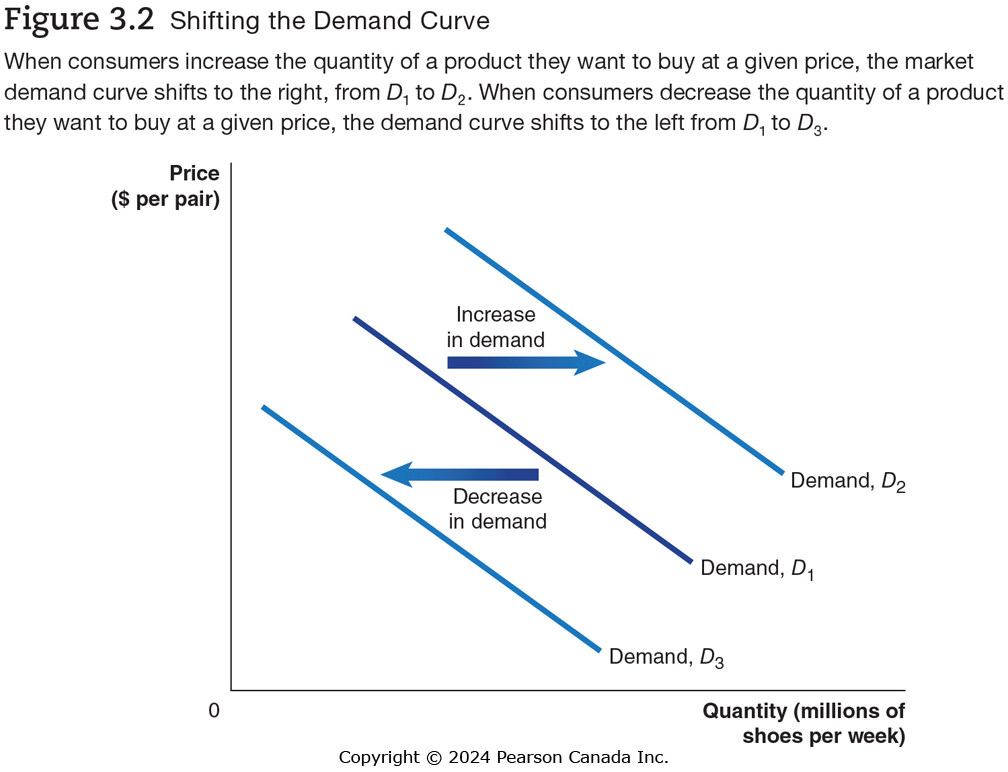
\includegraphics[width=0.6\linewidth]{Fig03-002}.
\end{frame}

\begin{frame}{Figure 3.2 -- Demand Shift vs.\ Quantity Demanded (2 of 2)}
\transfade
\begin{itemize}
  \item As the demand curve shifts, the quantity demanded will change, \textbf{even if the price does not change}.
  \item The quantity demanded changes at \textbf{every possible price}.
\end{itemize}
\end{frame}

\begin{frame}{Variables That Shift Market Demand}
\transfade
\begin{itemize}
  \item Income of consumers
  \item Prices of related goods
  \item Tastes
  \item Population and demographics
  \item Expectations
\end{itemize}
\end{frame}

\begin{frame}{Changes in Income of Consumers}
\transfade
\begin{itemize}
  \item \textbf{Normal goods:} goods for which demand increases as income rises and decreases as income falls.
  \begin{itemize}
    \item Examples: new clothes, restaurant meals, vacations.
  \end{itemize}
  \item \textbf{Inferior goods:} goods for which demand increases as income falls and decreases as income rises.
  \begin{itemize}
    \item Examples: second-hand clothes, instant noodles.
  \end{itemize}
\end{itemize}
\end{frame}

\begin{frame}{Effects of Changes in Income}
\transfade
\begin{itemize}
  \item An increase in income will:
  \begin{itemize}
    \item Increase the demand for new clothes (normal good), \emph{ceteris paribus}.
    \item Decrease the demand for second-hand clothes (inferior good).
  \end{itemize}
\end{itemize}
\end{frame}

\begin{frame}{Apply the Concept: Lobster as Inferior vs.\ Normal Good}
\transfade
\small
\begin{itemize}
  \item In some parts of the Maritimes, lobster is an \textbf{inferior good}: as incomes rise, people eat \emph{less} lobster.
  \item In large cities, lobster is a \textbf{normal good}: as incomes rise, people eat \emph{more} lobster.
  \item Key lesson:
  \begin{itemize}
    \item Whether a good is normal or inferior depends on \textbf{consumer behaviour} and context, not its intrinsic characteristics.
  \end{itemize}
\end{itemize}
\end{frame}

\begin{frame}{Changes in the Price of Related Goods}
\transfade
\begin{itemize}
  \item \textbf{Substitutes:} goods and services that can be used for the same purpose.
  \begin{itemize}
    \item Examples: Big Mac and Whopper; Ford F-150 and Dodge Ram; jeans and khakis.
  \end{itemize}
  \item \textbf{Complements:} goods and services that are used together.
  \begin{itemize}
    \item Examples: Big Mac and McDonald\'s fries; hot dogs and hot dog buns.
  \end{itemize}
\end{itemize}
\end{frame}

\begin{frame}{Effects of Changes in the Price of Related Goods}
\transfade
\begin{itemize}
  \item An increase in the price of a Big Mac:
  \begin{itemize}
    \item \textbf{Increases} the demand for Whoppers (substitute).
    \item \textbf{Decreases} the demand for McDonald\'s fries (complement).
  \end{itemize}
\end{itemize}
\end{frame}

\begin{frame}{Changes in Tastes}
\transfade
\begin{itemize}
  \item If consumers\' tastes change, they may buy more or less of a product.
  \item Example:
  \begin{itemize}
    \item If consumers become more concerned about healthy eating, they might decrease their demand for fast food.
  \end{itemize}
\end{itemize}
\end{frame}

\begin{frame}{Changes in Population and Demographics}
\transfade
\begin{itemize}
  \item \textbf{Demographics:} characteristics of a population (age, race, gender, etc.).
  \item Increases in the \textbf{number of people} buying something will increase the amount demanded.
  \item Example:
  \begin{itemize}
    \item An increase in the elderly population increases the demand for medical care.
  \end{itemize}
\end{itemize}
\end{frame}

\begin{frame}{Changes in Expectations About Future Prices}
\transfade
\begin{itemize}
  \item Consumers decide not only \textbf{which} products to buy but also \textbf{when} to buy them.
  \item Future products are \textbf{substitutes} for current products.
  \item An expected \textbf{increase} in price tomorrow \(\Rightarrow\) increases demand today.
  \item An expected \textbf{decrease} in price tomorrow \(\Rightarrow\) decreases demand today.
  \item Example: If you find out that the price of gasoline will go up tomorrow, you increase your demand today.
\end{itemize}
\end{frame}

\begin{frame}{Figure 3.3 -- Change in Demand vs.\ Change in Quantity Demanded}
\transfade
\begin{itemize}
  \item A change in the \textbf{price of the product itself} causes a \textbf{movement along} the demand curve:
  \begin{itemize}
    \item This is a \alert{change in quantity demanded}.
  \end{itemize}
  \item Any other change affecting demand causes the \textbf{entire demand curve to shift}:
  \begin{itemize}
    \item This is a \alert{change in demand}.
  \end{itemize}
\end{itemize}
\end{frame}

\begin{frame}{Figure 3.3 }
\centering
\vspace{1em}

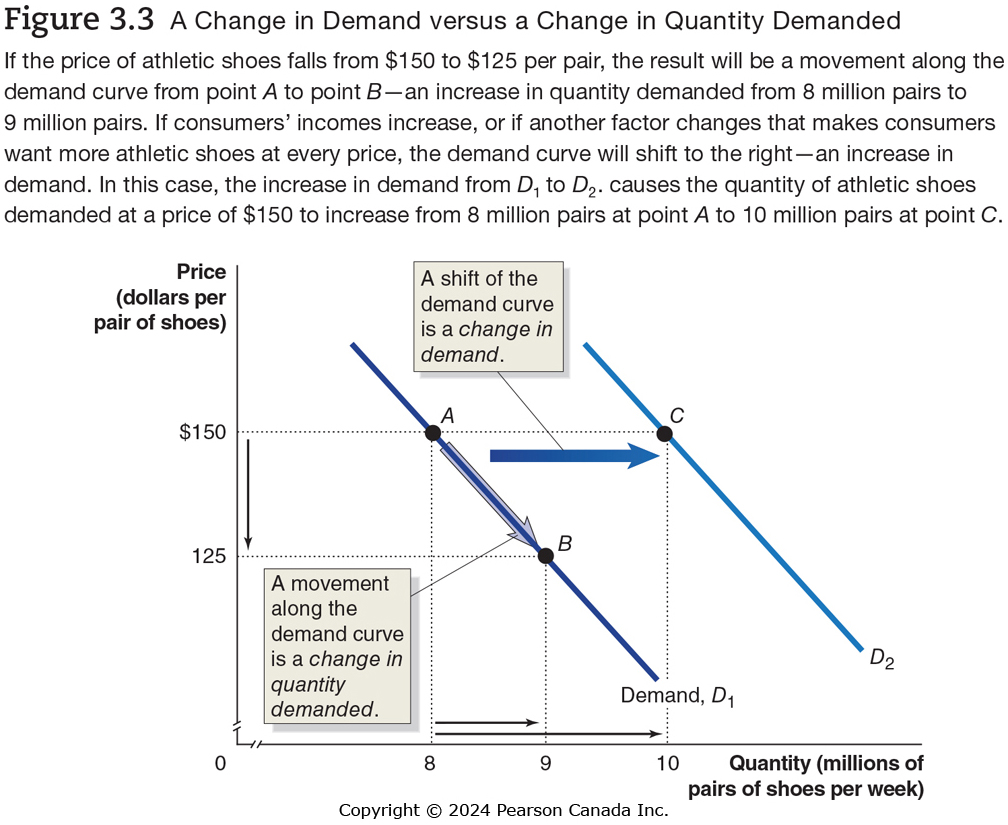
\includegraphics[width=0.56\linewidth]{Fig03-003}.
\end{frame}

% ============================================================
\section{The Supply Side of the Market (3.2)}
% ============================================================

\begin{frame}{3.2 Learning Objective}
\transfade
\begin{block}{Goal}
Discuss the variables that influence supply.
\end{block}
\begin{itemize}
  \item There are similarities and important differences between the demand and supply sides.
  \item Now we examine \textbf{market supply}: decisions of firms about how much of a product to provide at various prices.
\end{itemize}
\end{frame}

\begin{frame}{Figure 3.4 -- A Supply Schedule and Supply Curve (1 of 2)}
\transfade
\begin{itemize}
  \item \textbf{Supply schedule:} a table that shows the relationship between the price of a product and the quantity of the product supplied.
  \item \textbf{Supply curve:} a curve that shows the relationship between the price of a product and the quantity of the product supplied.
\end{itemize}
\end{frame}

\begin{frame}{Figure 3.4 -- Supply Schedule and Curve}
\centering


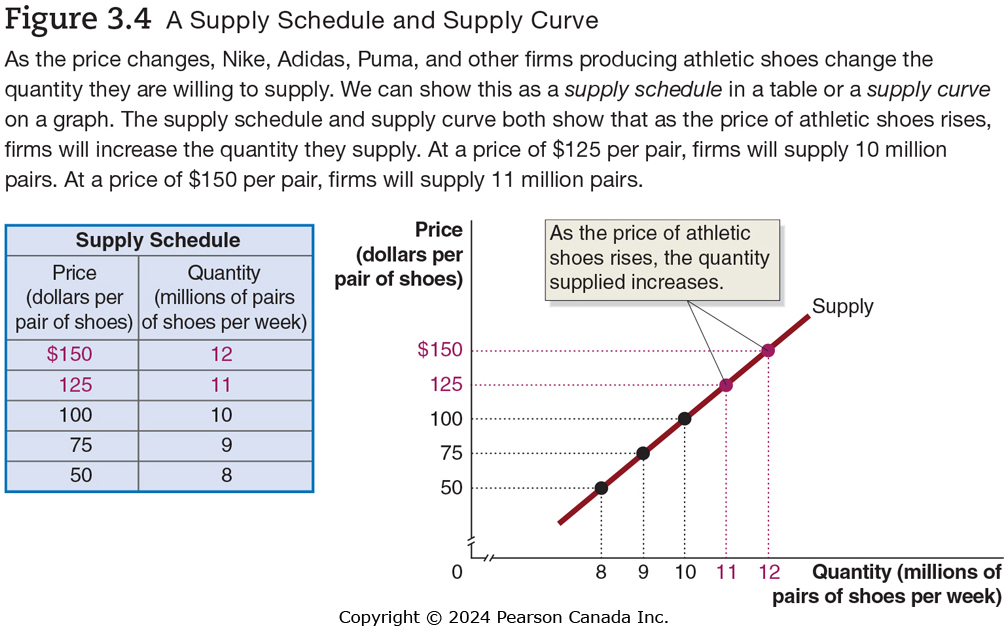
\includegraphics[width=0.75\linewidth]{Fig03-004}.
\end{frame}

\begin{frame}{Figure 3.4 -- Quantity Supplied and Law of Supply (2 of 2)}
\transfade
\begin{itemize}
  \item \textbf{Quantity supplied:} the amount of a good or service that a firm is willing and able to supply at a given price.
  \item \textbf{Law of supply:}
  \begin{itemize}
    \item Holding everything else constant, increases in price cause \textbf{increases} in quantity supplied.
    \item Decreases in price cause \textbf{decreases} in quantity supplied.
  \end{itemize}
\end{itemize}
\end{frame}

\begin{frame}{Figure 3.5 -- Shifting the Supply Curve (1 of 2)}
\transfade
\begin{itemize}
  \item A change in something \textbf{other than price} that affects supply causes the entire supply curve to \textbf{shift}.
  \item A shift to the right (\(S_1\) to \(S_3\)) is an \alert{increase in supply}.
  \item A shift to the left (\(S_1\) to \(S_2\)) is a \alert{decrease in supply}.
\end{itemize}
\end{frame}

\begin{frame}{Figure 3.5 -- Shifting the Supply Curve }
\centering


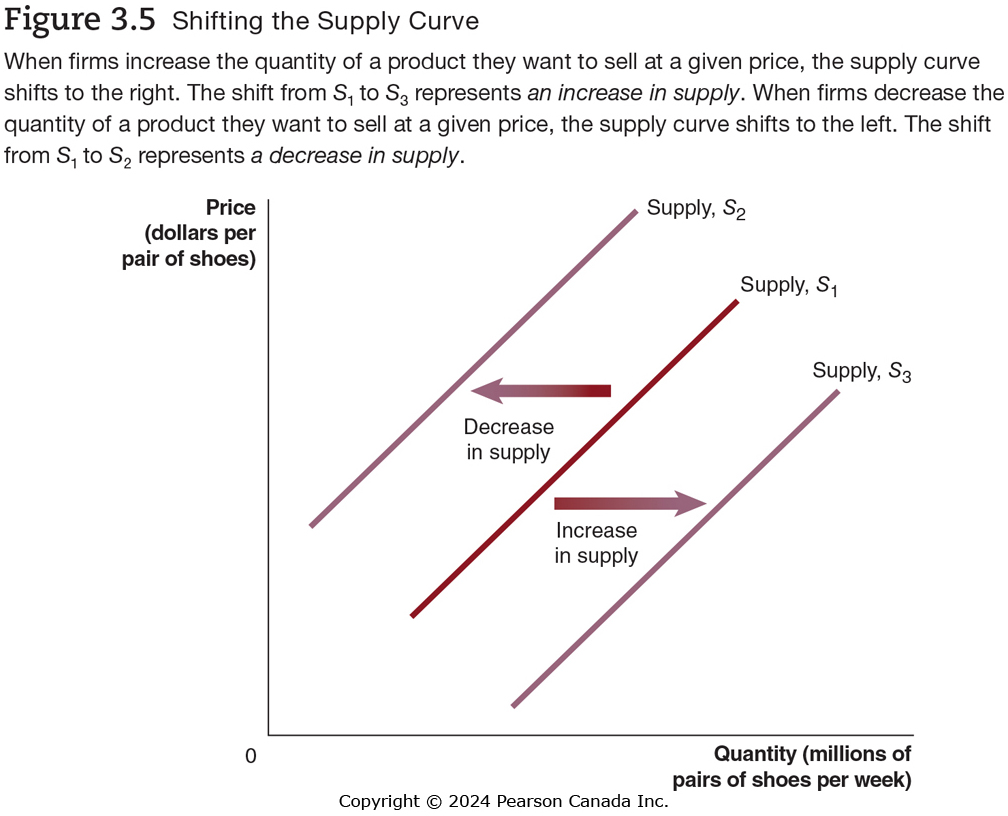
\includegraphics[width=0.6\linewidth]{Fig03-005}.
\end{frame}

\begin{frame}{Figure 3.5 -- Supply Shift vs.\ Quantity Supplied (2 of 2)}
\transfade
\begin{itemize}
  \item As the supply curve shifts, the quantity supplied changes \textbf{even if the price does not change}.
  \item The quantity supplied changes at every possible price.
\end{itemize}
\end{frame}

\begin{frame}{Variables That Shift Market Supply}
\transfade
\begin{itemize}
  \item Prices of inputs
  \item Technological change
  \item Prices of substitutes in production
  \item Number of firms in the market
  \item Expected future prices
\end{itemize}
\end{frame}

\begin{frame}{Changes in Prices of Inputs}
\transfade
\begin{itemize}
  \item \textbf{Inputs} are anything used in the production of a good or service.
  \begin{itemize}
    \item For athletic shoes: rubber, plastic, and labour.
  \end{itemize}
  \item An \alert{increase} in the price of an input decreases the profitability of selling the good, causing a \textbf{decrease in supply}.
  \item A \alert{decrease} in the price of an input increases profitability, causing an \textbf{increase in supply}.
\end{itemize}
\end{frame}

\begin{frame}{Technological Change}
\transfade
\begin{itemize}
  \item A firm may experience a positive or negative change in its ability to produce a given level of output with a given quantity of inputs.
  \item This is called \textbf{technological change}.
  \item Examples:
  \begin{itemize}
    \item A new, more efficient way of producing shoes \(\Rightarrow\) \textbf{increases} supply.
    \item Government restrictions on how much workers can work \(\Rightarrow\) \textbf{decreases} supply.
  \end{itemize}
\end{itemize}
\end{frame}

\begin{frame}{Prices of Substitutes and Complements in Production}
\transfade
\begin{itemize}
  \item Many firms can produce and sell alternative products: \textbf{substitutes in production}.
  \item Example:
  \begin{itemize}
    \item An Ontario farmer can plant either corn or soybeans.
    \item If the price of soybeans rises, the farmer will plant (supply) less corn.
  \end{itemize}
  \item Sometimes two products are necessarily produced together: \textbf{complements in production}.
  \item Example:
  \begin{itemize}
    \item Cattle provide both beef and leather.
    \item An increase in the price of beef encourages more cattle farming, which increases the supply of leather.
  \end{itemize}
\end{itemize}
\end{frame}

\begin{frame}{Number of Firms and Expected Future Prices}
\transfade
\begin{itemize}
  \item More firms in the market \(\Rightarrow\) more product available at a given price (greater supply).
  \item If a firm anticipates that the price of its product will be \textbf{higher} in the future, it might \textbf{decrease} its supply today to increase it in the future.
\end{itemize}
\end{frame}

\begin{frame}{Figure 3.6 -- Change in Supply vs.\ Change in Quantity Supplied}
\transfade
\begin{itemize}
  \item A change in the \textbf{price of the product itself} causes a \textbf{movement along} the supply curve:
  \begin{itemize}
    \item This is a \alert{change in quantity supplied}.
  \end{itemize}
  \item Any other change affecting supply shifts the entire supply curve:
  \begin{itemize}
    \item This is a \alert{change in supply}.
  \end{itemize}
\end{itemize}
\end{frame}

\begin{frame}{Figure 3.6 }
\centering


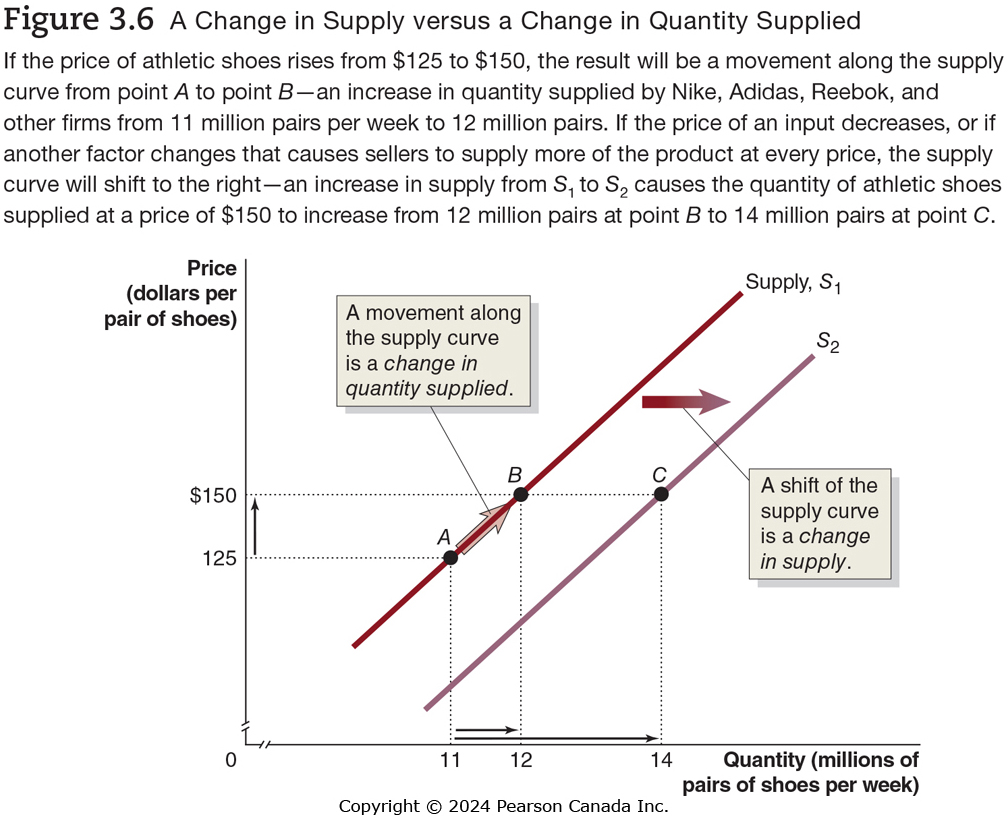
\includegraphics[width=0.6\linewidth]{Fig03-006}.
\end{frame}

% ============================================================
\section{Market Equilibrium (3.3)}
% ============================================================

\begin{frame}{3.3 Learning Objective}
\transfade
\begin{block}{Goal}
Use a graph to illustrate market equilibrium.
\end{block}
\begin{itemize}
  \item \textbf{Market equilibrium:} quantity demanded equals quantity supplied.
  \item In markets with many buyers and sellers (perfectly competitive), we call this a \textbf{competitive market equilibrium}.
\end{itemize}
\end{frame}

\begin{frame}{Figure 3.7 -- Market Equilibrium (Athletic Shoes)}
\transfade
\begin{itemize}
  \item Consider the market for athletic shoes.
  \item At a price of \$100:
  \begin{itemize}
    \item Consumers want to buy 10 million pairs of shoes per week.
    \item Producers want to sell 10 million pairs of shoes per week.
  \end{itemize}
  \item The \textbf{equilibrium price} is \$100, and the \textbf{equilibrium quantity} is 10 million pairs per week.
\end{itemize}
\end{frame}

\begin{frame}{Figure 3.7 -- Market Equilibrium}
\centering


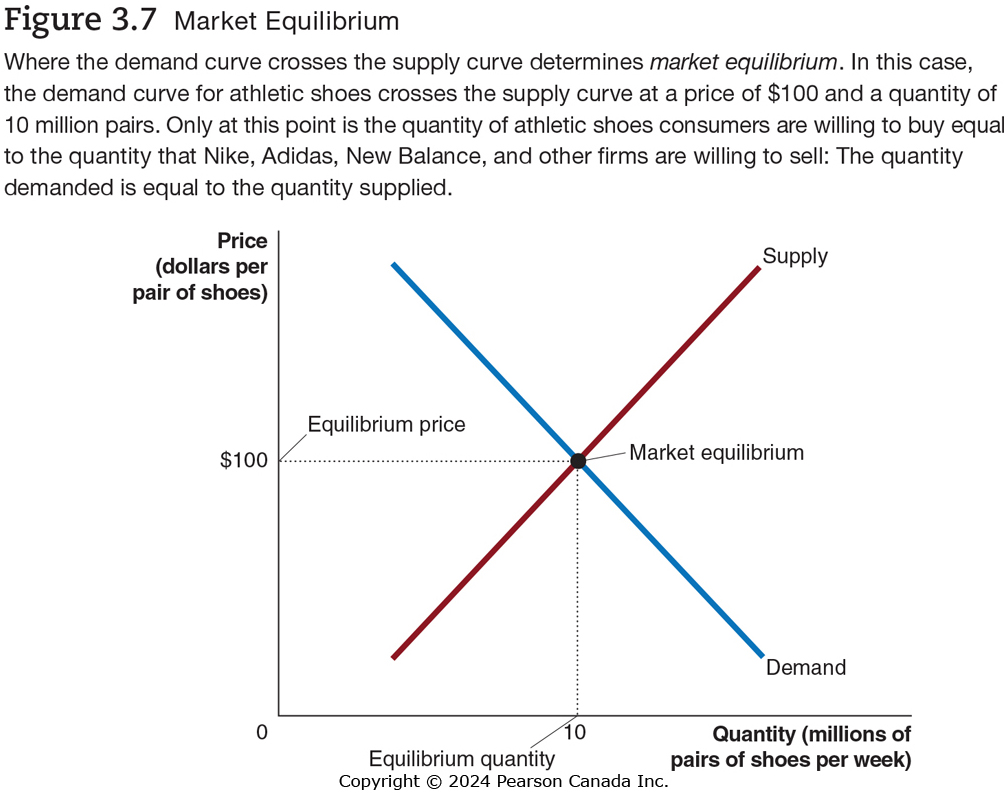
\includegraphics[width=0.6\linewidth]{Fig03-007}.
\end{frame}

\begin{frame}{Figure 3.8 -- Surpluses and Shortages (1 of 2)}
\transfade
\begin{itemize}
  \item What if the price were \$125 instead?
  \item At \$125:
  \begin{itemize}
    \item Consumers want to buy 9 million pairs of shoes.
    \item Producers want to sell 11 million pairs of shoes.
  \end{itemize}
  \item This gives a \textbf{surplus} of 2 million pairs: quantity supplied exceeds quantity demanded.
  \item Prediction: sellers will compete among themselves, driving the price \textbf{down} toward equilibrium.
\end{itemize}
\end{frame}

\begin{frame}{Figure 3.8 -- Surplus}
\centering


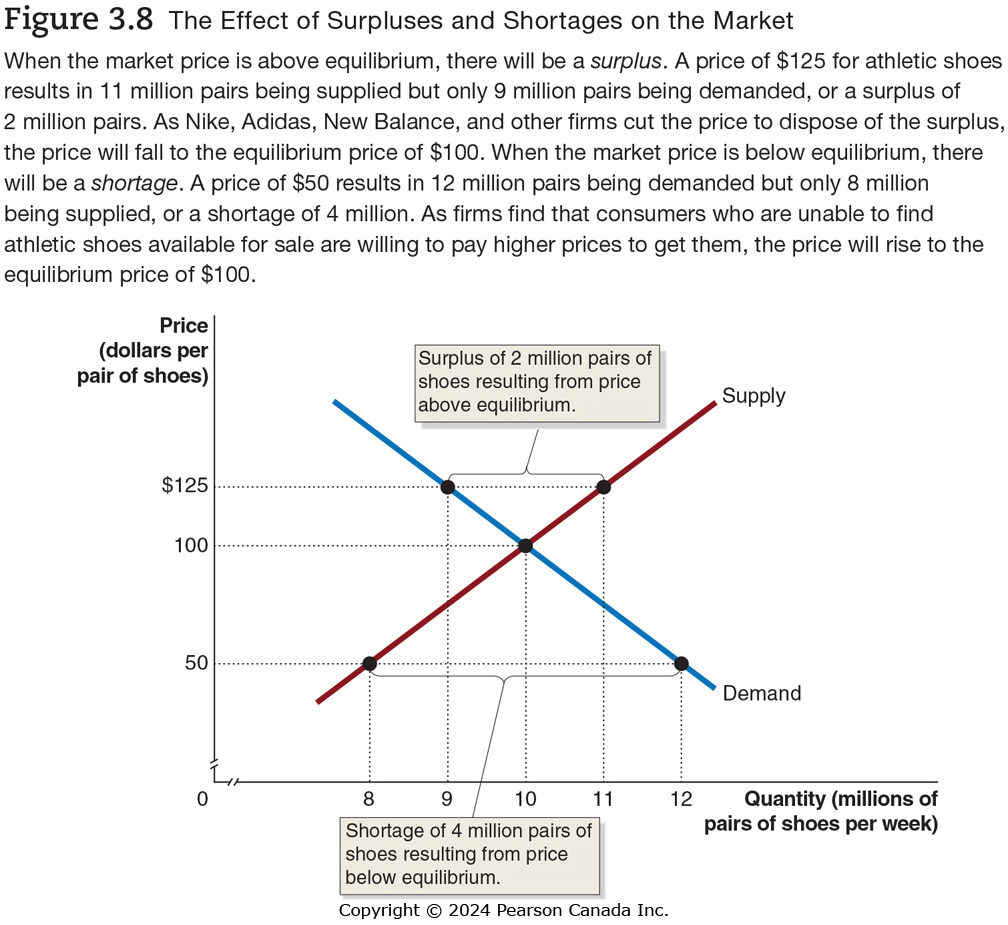
\includegraphics[width=0.55\linewidth]{Fig03-008}.
\end{frame}

\begin{frame}{Figure 3.8 -- Surpluses and Shortages (2 of 2)}
\transfade
\begin{itemize}
  \item What if the price were \$50?
  \item At \$50:
  \begin{itemize}
    \item Consumers want to buy 12 million pairs of shoes.
    \item Producers want to sell 8 million pairs.
  \end{itemize}
  \item This gives a \textbf{shortage} of 4 million pairs: quantity demanded exceeds quantity supplied.
  \item Prediction: sellers realize they can increase price and still sell as many pairs \(\Rightarrow\) price will \textbf{rise} toward equilibrium.
\end{itemize}
\end{frame}

\begin{frame}{Figure 3.8 -- Shortage }
\centering


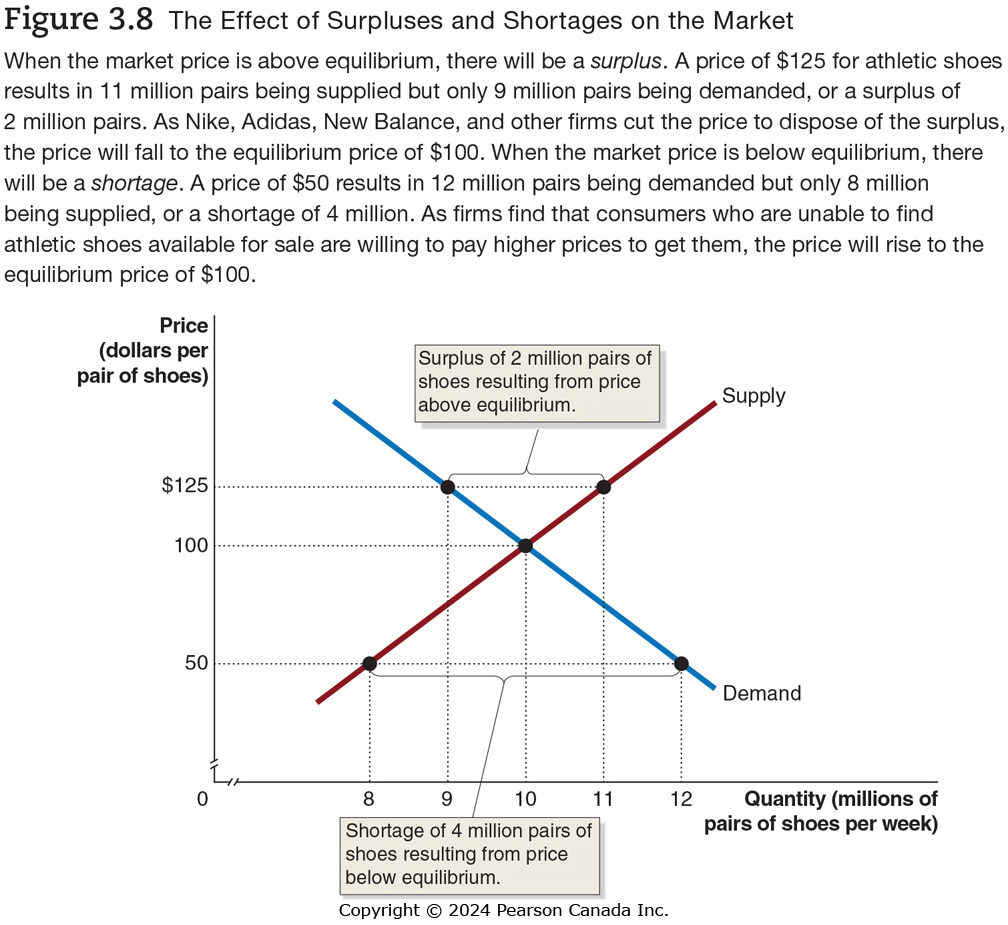
\includegraphics[width=0.55\linewidth]{Fig03-008}.
\end{frame}

\begin{frame}{Demand and Supply Both Count}
\transfade
\begin{itemize}
  \item Price is determined by the \textbf{interaction} of buyers and sellers.
  \item In a competitive market, neither group alone can dictate the price.
  \item However, \textbf{changes in demand and/or supply} will affect the equilibrium price and quantity traded.
\end{itemize}
\end{frame}

% ============================================================
\section{Shifts in Demand and Supply (3.4)}
% ============================================================

\begin{frame}{3.4 Learning Objective}
\transfade
\begin{block}{Goal}
Use demand and supply graphs to predict changes in prices and quantities.
\end{block}
\begin{itemize}
  \item We typically know the actual price and quantity, but do \emph{not} observe the whole curves.
  \item The power of the model is in predicting \textbf{directional changes} in price and quantity when curves shift.
\end{itemize}
\end{frame}

\begin{frame}{Figure 3.9 -- Effect of an Increase in Supply (1 of 2)}
\transfade
\begin{itemize}
  \item Market for athletic shoes when a new shoemaker enters the market.
  \item At any given price, more shoes are supplied:
  \begin{itemize}
    \item Supply shifts right from \(S_1\) to \(S_2\).
  \end{itemize}
  \item \textbf{Result:}
  \begin{itemize}
    \item Equilibrium price \textbf{falls}.
    \item Equilibrium quantity \textbf{rises}.
  \end{itemize}
\end{itemize}
\end{frame}

\begin{frame}{Figure 3.9 -- Increase in Supply}
\centering
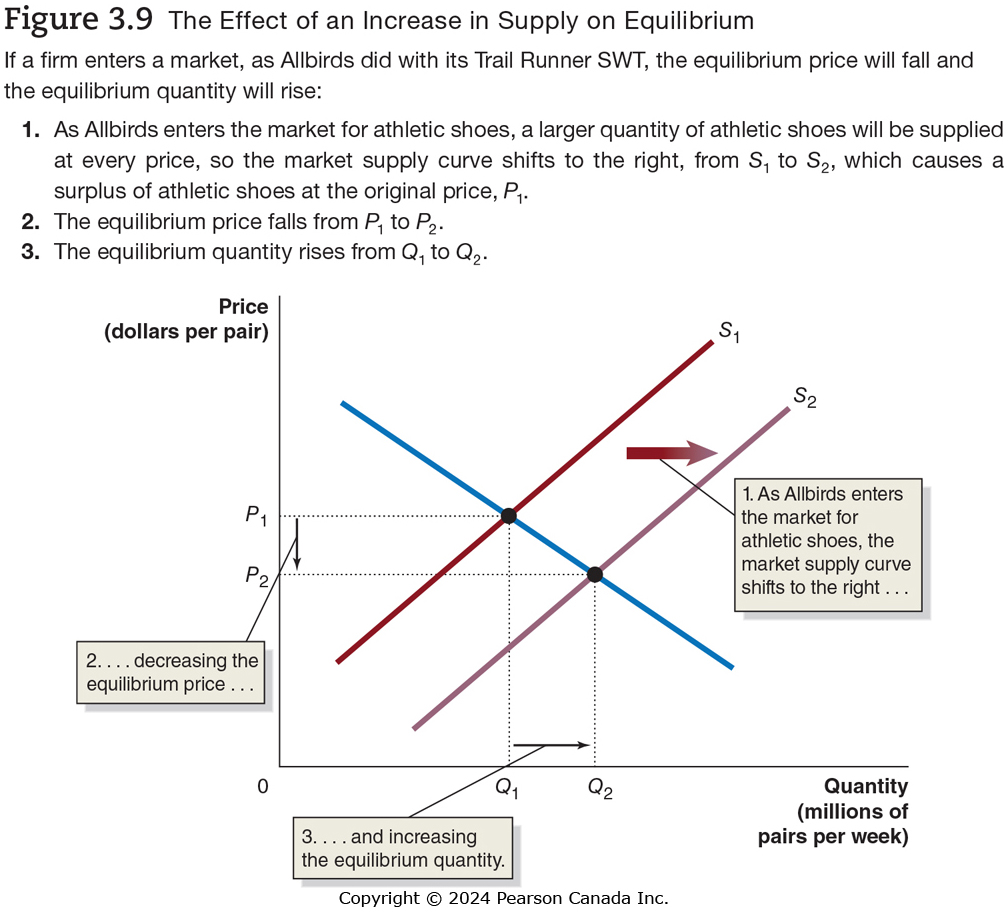
\includegraphics[width=0.55\linewidth]{Fig03-009}.
\end{frame}

\begin{frame}{Figure 3.9 -- How Much Does Price Fall? (2 of 2)}
\transfade
\begin{itemize}
  \item By how much will price fall?
  \item By how much will quantity rise?
  \item We \textbf{cannot} say without knowing more (the exact shapes and positions of demand and supply).
  \item For now, we only predict \emph{directions}: price falls, quantity rises.
\end{itemize}
\end{frame}

\begin{frame}{Figure 3.10 -- Effect of an Increase in Demand}
\transfade
\begin{itemize}
  \item Suppose incomes increase.
  \item Athletic shoes are a \textbf{normal good}, so as income rises, demand shifts to the right.
  \item \textbf{Result:}
  \begin{itemize}
    \item Equilibrium price \textbf{rises}.
    \item Equilibrium quantity \textbf{rises}.
  \end{itemize}
\end{itemize}
\end{frame}

\begin{frame}{Figure 3.10 -- Increase in Demand }
\centering
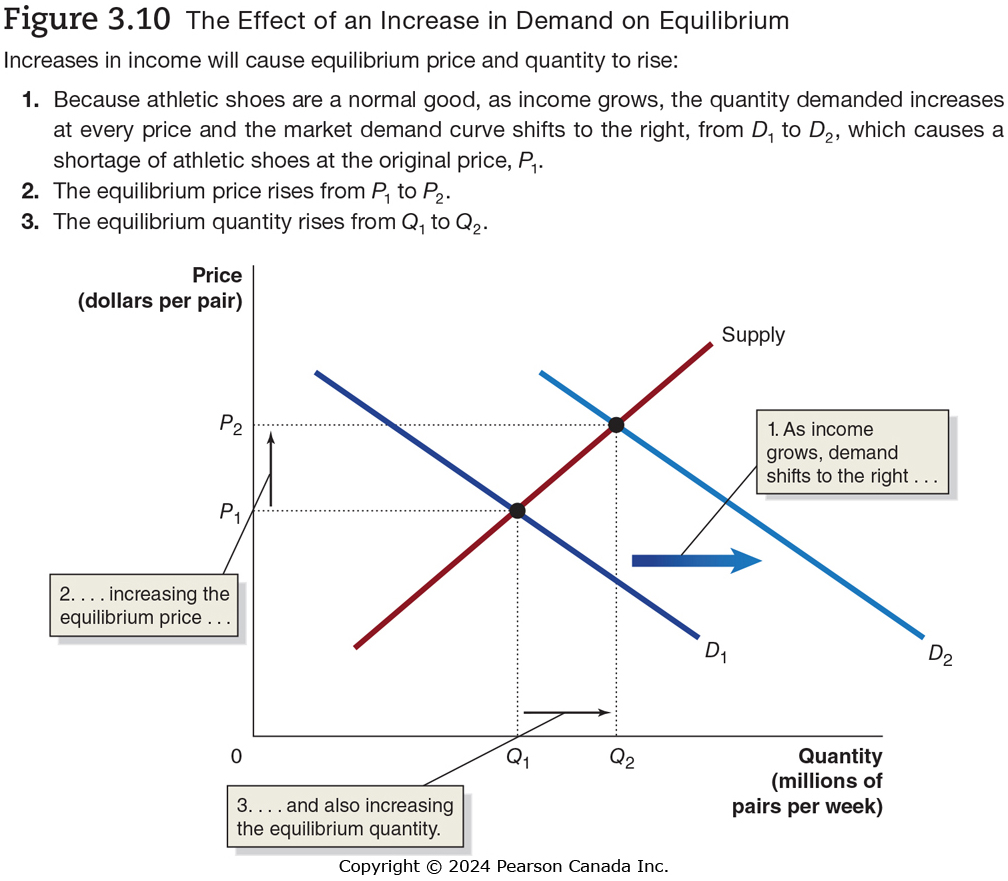
\includegraphics[width=0.55\linewidth]{Fig03-010}.
\end{frame}

\begin{frame}{Table 3.3 -- How Shifts in Demand and Supply Affect Equilibrium \(P\) and \(Q\) (1 of 2)}
\transfade
\small
\begin{tabular}{>{\bfseries}lcc}
\toprule
 & Equilibrium Price \(P\) & Equilibrium Quantity \(Q\) \\
\midrule
Increase in demand, supply unchanged & Rises & Rises \\
Decrease in demand, supply unchanged & Falls & Falls \\
Increase in supply, demand unchanged & Falls & Rises \\
Decrease in supply, demand unchanged & Rises & Falls \\
\bottomrule
\end{tabular}
\end{frame}

\begin{frame}{Table 3.3 -- How Shifts in Demand and Supply Affect \(P\) and \(Q\) (2 of 2)}
\transfade
\small
\begin{tabular}{>{\bfseries}lcc}
\toprule
 & Equilibrium Price \(P\) & Equilibrium Quantity \(Q\) \\
\midrule
\textcolor{accent}{Increase in supply, demand unchanged} & \textcolor{accent}{Falls} & \textcolor{accent}{Rises} \\
Increase in demand, decrease in supply & Rises & ? \\
Decrease in demand, increase in supply & Falls & ? \\
Increase in demand, increase in supply & ? & Rises \\
Decrease in demand, decrease in supply & ? & Falls \\
\bottomrule
\end{tabular}

\vspace{0.5em}
\begin{itemize}
  \item The highlighted row (in blue text) is the example we studied: \textbf{increase in supply}.
  \item ``?'' means the effect is \textbf{ambiguous} without more information on the relative size of shifts.
\end{itemize}
\end{frame}

\begin{frame}{Figure 3.11 -- Shifts in Demand and Supply Over Time (1 of 3)}
\transfade
\begin{itemize}
  \item Over time, it is likely that \textbf{both} demand and supply will change.
  \item Example:
  \begin{itemize}
    \item New firms enter \(\Rightarrow\) supply shifts right.
    \item Incomes rise \(\Rightarrow\) demand shifts right.
  \end{itemize}
\end{itemize}
\end{frame}

\begin{frame}{Figure 3.11 -- Both Demand and Supply Shift}
\centering
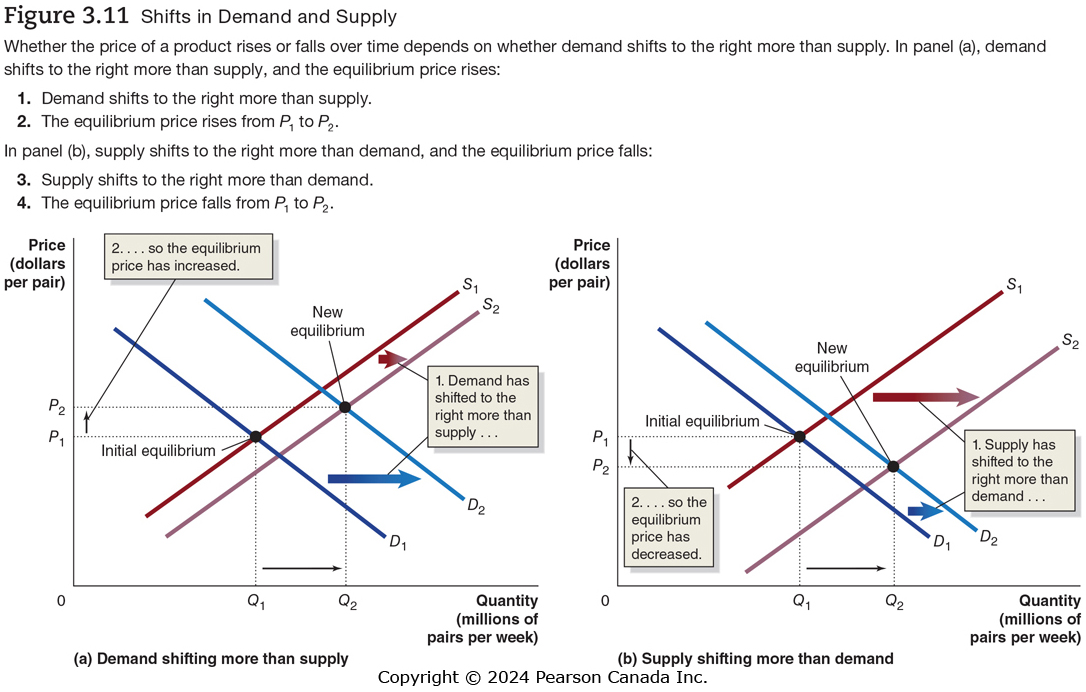
\includegraphics[width=0.78\linewidth]{Fig03-011}.
\end{frame}

\begin{frame}{Figure 3.11 -- Case 1: Demand Shifts More than Supply (2 of 3)}
\transfade
\begin{itemize}
  \item When demand shifts more than supply:
  \begin{itemize}
    \item Equilibrium quantity \textbf{rises}.
    \item Equilibrium price also \textbf{rises}.
  \end{itemize}
  \item This panel shows a larger rightward shift of demand than of supply.
\end{itemize}
\end{frame}

\begin{frame}{Figure 3.11 -- Case 2: Supply Shifts More than Demand (3 of 3)}
\transfade
\begin{itemize}
  \item When supply shifts more than demand:
  \begin{itemize}
    \item Equilibrium quantity \textbf{rises}.
    \item Equilibrium price \textbf{falls}.
  \end{itemize}
  \item Without knowing the relative size of the changes, the effect on price is ambiguous.
  \item It is possible, but unlikely, that equilibrium price remains unchanged.
\end{itemize}
\end{frame}

\begin{frame}{Shifts of Curves vs.\ Movements Along Curves}
\transfade
\begin{itemize}
  \item Suppose an \textbf{increase in supply} occurs.
  \item We know:
  \begin{itemize}
    \item Equilibrium quantity will increase.
    \item Equilibrium price will decrease.
  \end{itemize}
  \item It is tempting to say ``the decrease in price causes an increase in demand'', but this is incorrect.
  \item The decrease in price causes a \textbf{movement along the demand curve}, not a shift of the curve.
  \item The demand curve already describes how much consumers want to buy at \textbf{any given price}.
\end{itemize}
\end{frame}

% ============================================================
\section{Chapter Summary}
% ============================================================

\begin{frame}{Summary}
\transfade
\begin{itemize}
  \item Demand:
  \begin{itemize}
    \item Follows the law of demand; explained by substitution and income effects.
    \item Shifts when income, prices of related goods, tastes, population, or expectations change.
  \end{itemize}
  \item Supply:
  \begin{itemize}
    \item Follows the law of supply.
    \item Shifts when input prices, technology, related goods in production, number of firms, or expected future prices change.
  \end{itemize}
  \item Market equilibrium:
  \begin{itemize}
    \item Occurs where quantity demanded equals quantity supplied.
    \item Surpluses cause price to fall; shortages cause price to rise.
  \end{itemize}
  \item The demand and supply model predicts \textbf{directional} changes in equilibrium price and quantity when curves shift.
\end{itemize}
\end{frame}

% ============================================================
\begin{frame}
\centering
\Huge \textbf{Thank you!}
\end{frame}

\end{document}
